\documentclass[12pt]{report}
\usepackage[left=1.5cm, right=1.5cm, top=2cm]{geometry}
\usepackage{graphicx}
\usepackage{imakeidx}

\renewcommand{\thesection}{Chapter \arabic{section}}
\renewcommand{\thesubsection}{\arabic{section}.\arabic{subsection}}

\begin{document}




\section{Background And Motivation}


\paragraph{ }
This Project presents the practices to follow during Software Development Lifecycle (SDLC).Scope of the project is to propose methods to incorporate security in software during each phase of SDLC to develop software which is resilient to attacks.

\subsection{Introduction To Software Development Lifecycle}
\paragraph{ }
Software Development Life Cycle (SDLC) is a process used by the software industry to design, develop and test high quality softwares. The SDLC aims to produce a high-quality software that meets or exceeds customer expectations, reaches completion within times and cost estimates.\par
    SDLC is a process followed for a software project, within a software organization. It consists of a detailed plan describing how to develop, maintain, replace and alter or enhance specific software. The life cycle defines a methodology for improving the quality of software and the overall development process.\par
    Following figure represents various stages in SDLC\\
\begin{figure}[h!]
	\begin{center}
		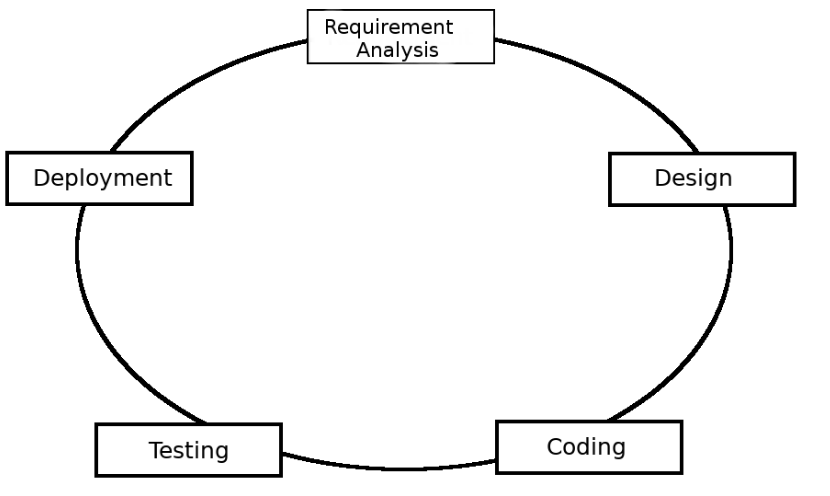
\includegraphics[scale =0.4]{images/sdlc.png}
		\caption{Software Devlopment Lifecycle}
		\label{sdlc}
	\end{center}
\end{figure}


\section{Another section}

\end{document}
